% !TEX root = ./main.tex
% !TEX encoding = UTF-8 Unicode
% !TEX program = pdflatex
% !TeX spellcheck = it_IT

\graphicspath{{Immagini/},{Immagini/android_aging/}}

\chapter{Software Aging on Android 7}

\section{Traccia}
Verificare se \textbf{Android} è soggetto ad \textbf{\textit{aging}}.\\

\section{System Under Test}
Il dispositivo utilizzato è un \textbf{Huawei P9 Lite}, con le seguenti caratteristiche:

\begin{itemize}
  \item \textbf{Chipset: }Kirin 650 (4 x 2,0GHz + 4 x 1,7GHZ) 64 bit
  \item \textbf{Memoria: } 3GB RAM, 16GB EMMC Flash ROM
  \item \textbf{Sistema Operativo: }Android 7.0
\end{itemize}

\section{Experimental Plan}

Per verificare il fenomeno dell'\textbf{Aging} sarà analizzato il \textbf{Lunch Time(LT)},
misura del tempo tra il click sull'icona dell'applicazione e l'avvio della stessa,
in quanto il fenomeno dell'aging, dal punto di vista dell'utente, è percepito
come una bassa reattività del dispositivo.\\
Gli indicatori di aging del sistema sono invece parametri che riguardano la \textit{memoria},
la \textit{Garbage Collection} ed il \textit{Task-Level}.\\

\section{Experimental Setup}

Gli esperimenti sono stati eseguiti su uno smartphone \textit{Huawei P9 Lite}, descritto
in precedenza, utilizzando il tool \textit{\textbf{ADB(Android Debug Bridge)}}.\\
La generazione del workload è stata effettuata tramite il tool
\textit{\textbf{Monkey WL generator}}, mentre la raccolta dei dati tramite le
utility \textit{\textbf{dumpsys}} e \textit{\textbf{logcat}}.\\
In figura \ref{and_setup} è riportato lo schema di connessione con il quale sono stati
eseguiti gli esperimenti.\\
La connessione tra PC e smartphone è stata realizzata tramite WiFi, quindi è
stato generato il workload tramite \textit{\textbf{Monkey WL generator}}, inviato
tramite WiFi al dispositivo mobile ed infine i dati sono stati raccolti
utilizzando \textit{\textbf{dumpsys}} e \textit{\textbf{logcat}}.\\

\begin{figure}[!htbp]
  \centering
  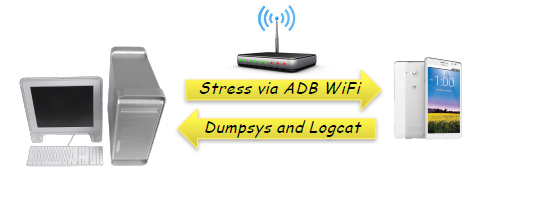
\includegraphics[width=\linewidth, keepaspectratio]{setup}
  \caption{Setup esperimenti}
  \label{and_setup}
\end{figure}

In totale sono stati eseguiti due test:
\begin{itemize}
  \item \textbf{Workload Fisso};
  \item \textbf{Workload Variabile}.
\end{itemize}

Il primo esperimento è un test di durata di 6 ore, cui obiettivo è stressare il
dispositivo effettuando un'operazione ogni 100ms.\\
Il secondo esperimento è un test che punta ad osservare il comportamento del dispositivo
in un utilizzo normale, con il tipico carico di un utente medio, effettuando
delle operazioni ad intervallo di tempo variabile(500ms, 1500ms e 2500ms).\\
Questo secondo test a workload variabile, sovraccaricando meno il sistema, ha una
durata complessiva di 12 ore.\\
In generale, in entrambi i test, il workload genera i seguenti movimenti
\begin{itemize}
  \item \textbf{Touch, Motion and Trackballs (33\%)};
  \item \textbf{(minor and major) Navigation (33\%)};
  \item \textbf{AppSwitch (34\%)}.
\end{itemize}
Le applicazioni utilizzate per gli esperimenti, riportate nella tabella in figura
\ref{and_applicazioni}, sono state ottenute lanciando il comando
\textit{adb shell pm list packages}.\\

\begin{figure}[!htbp]
  \centering
  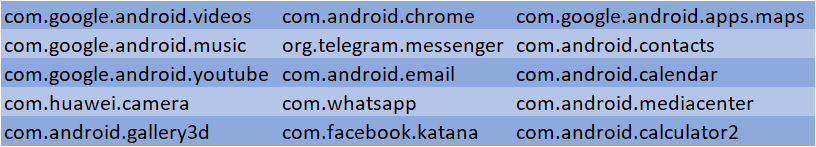
\includegraphics[width=\linewidth, keepaspectratio]{applicazioni}
  \caption{Applicazioni Workload}
  \label{and_applicazioni}
\end{figure}

L'esecuzione degli esperimenti è stata effettuata lanciando lo script bash
\textit{\textbf{runtest.sh}} il quale richiama i seguenti script:
  \begin{itemize}
    \item \textit{\textbf{logcat\_art.sh}}: raccoglie i dati relativi al \textit{Garbage Collector};
    \item \textit{\textbf{dumpTask.sh}}: raccoglie i dati relativi ai task;
    \item \textit{\textbf{dumpOnlyMeminfo.sh}}: raccoglie i dati relativi alla memoria;
    \item \textit{\textbf{loagcat\_displayed.sh}}: raccoglie i dati relativi al LT;
    \item \textit{\textbf{kill\_after\_time.sh}}: permette di definire il tempo di
    sperimentazione ed esegue il reboot in modalità recovery del dispositivo;
    \item \textit{\textbf{LaunchTimeMeasurement.sh}}: esegue lo stress test del dispositivo;
    \item \textit{\textbf{WorkloadFixed.sh o WorkloadVariable.sh}}: il primo definisce le applicazioni del
    workload fisso, il secondo definisce l'esecuzione del workload variabile, richiamando
    a sua volta ulteriori 3 script, nei quali sono definite le applicazioni da lanciare.
  \end{itemize}

\section{Data Analysis}

L'esecuzione dello script \textbf{\textit{runtest.sh}} genera diversi file di log
tra cui \textit{\textbf{Displyed.txt}} e \textit{\textbf{meminfo.txt}}, i quali
contengono rispettivamente i dati relativi ai tempi di lancio delle activity ed
i dati relativi all'utilizzo della memoria.\\
L'analisi relativa ai tempi di lancio è effettuata tramite lo script \textbf{\textit{generate\_Time\_data.sh}},
il quale estrae una serie temporale per ogni activity, sulla quale effettua,
tramite un script R, il \textbf{\textit{Mann Kendall test}} con intervallo
di confidenza al 90\%.\\
Il \textbf{\textit{Mann Kendall test}} è un test che mira a verificare l'esistenza
di un trend nei dati.\\
Valori bassi del p-value rifiutano $H_0$, ovvero l'esistenza del trend.\\
Inoltre lo script genera i plot per ogni activity.\\
L'analisi relativa alla memoria è effettuata tramite i seguenti script:
\begin{itemize}
  \item \textit{\textbf{generate\_Meminfo\_data.sh}}:
  \item \textit{\textbf{generate\_Global\_Meminfo\_data.sh}}: genera le statistiche
  globali per i parametri di memoria RAM e i relativi plot temporali;
  \item \textit{\textbf{generate\_Meminfo\_data\_Slopes.sh}}: esegue il \textbf{\textit{Mann Kendal test}}
  per ogni task attivo sul dispositivo;
\end{itemize}

\clearpage

\subsection{Launch Time Analysis(Worklaod Fixed)}
Dopo aver analizzato i valori di \textit{slope}(pendenza della retta) e
\textit{p-value}(relativo al Mann Kendall test), si osserva, in figura \ref{and_analisi_trend_lt_activity_1},
che alcune activity presentano un trend positivo, anche se la crescita
del loro LT non è significativa poiché il valore slope non è sufficientemente
alto.\\
Quanto affermato è validato dai i plot ottenuti eseguendo lo script
\textit{\textbf{generate\_Meminfo\_data.sh}}.

\begin{figure}[!htbp]
  \centering
  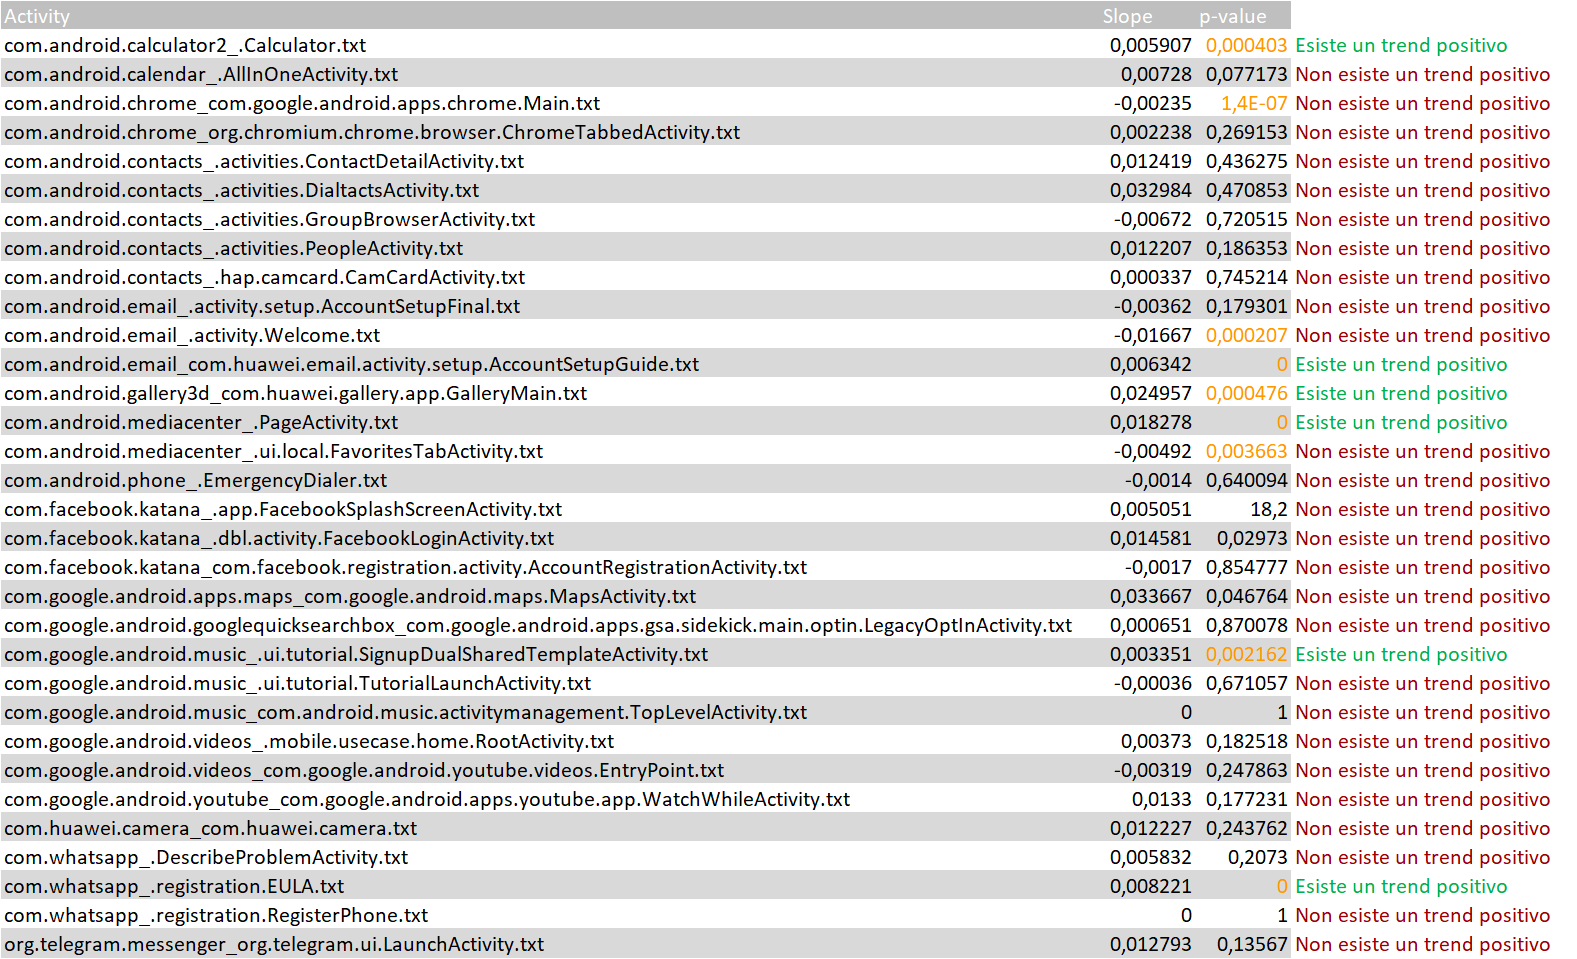
\includegraphics[width=\linewidth, keepaspectratio]{analisi_trend_lt_activity_1}
  \caption{Trend Activity Workload Fixed}
  \label{and_analisi_trend_lt_activity_1}
\end{figure}

\clearpage

\subsection{Launch Time Analysis(Worklaod Variable)}
Dopo aver analizzato i valori di \textit{slope}(pendenza della retta) e
\textit{p-value}(relativo al Mann Kendall test), si osserva, in figura \ref{and_analisi_trend_lt_activity_2},
che alcune activity presentano un trend positivo, anche se la crescita
del loro LT non è significativa poiché il valore slope non è sufficientemente
alto.\\
Quanto affermato è validato dai i plot ottenuti eseguendo lo script
\textit{\textbf{generate\_Meminfo\_data.sh}}.

\begin{figure}[!htbp]
  \centering
  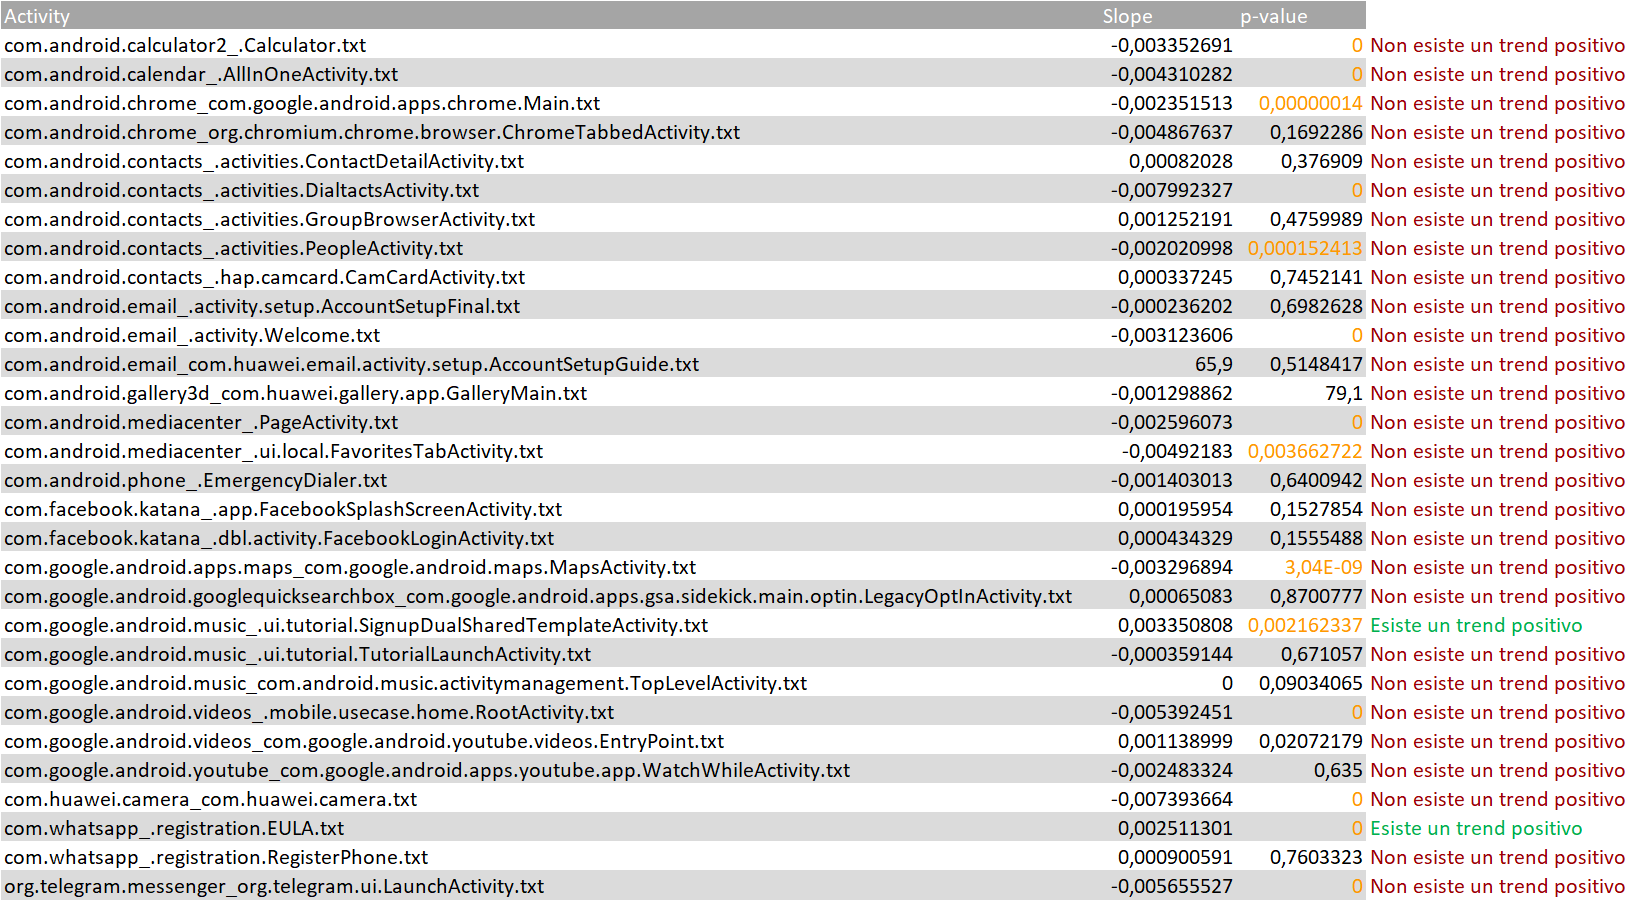
\includegraphics[width=\linewidth, keepaspectratio]{analisi_trend_lt_activity_2}
  \caption{Trend Activity Workload Fixed}
  \label{and_analisi_trend_lt_activity_2}
\end{figure}

\clearpage

\subsection{Memory Analysis(Worklaod Fixed)}

Nell'analisi a basso livello verrà considerato il parametro PSS(Proportional Set Size)
dei processi \textit{system}, \textit{systemui}, \textit{mediaserver} e
\textit{surfaceflinger}, per i quali sarà verificata l'esistenza di un trend.\\

\begin{figure}[!htbp]
  \centering
  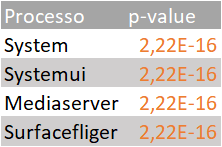
\includegraphics[width=.3\linewidth, keepaspectratio]{pvalue_memoria_1}
  \caption{System}
  \label{and_pvalue_memoria_1}
\end{figure}

Nella tabella in figura \ref{and_pvalue_memoria_1} sono riportati i p-value associati
al \textit{Mann Kendall test}.\\
Quest'ultimo suggerisce che può essere rigettata l'ipotesi nulla, dimostrando
che in tutte le serie temporali esiste un trend.\\
In particolare, osservando le immagini in figura \ref{and_minipage_trends}, si verifica che effettivamente
tutti i processi presentano un trend, in particolare \textit{mediaserver},
il quale presenta un trend negativo.\\
Il trend più significativo è verificato nei processi \textit{system} e \textit{systemui}.

\begin{minipage}{\linewidth}
  \centering
  \begin{minipage}{0.49\linewidth}
    \begin{figure}[H]
      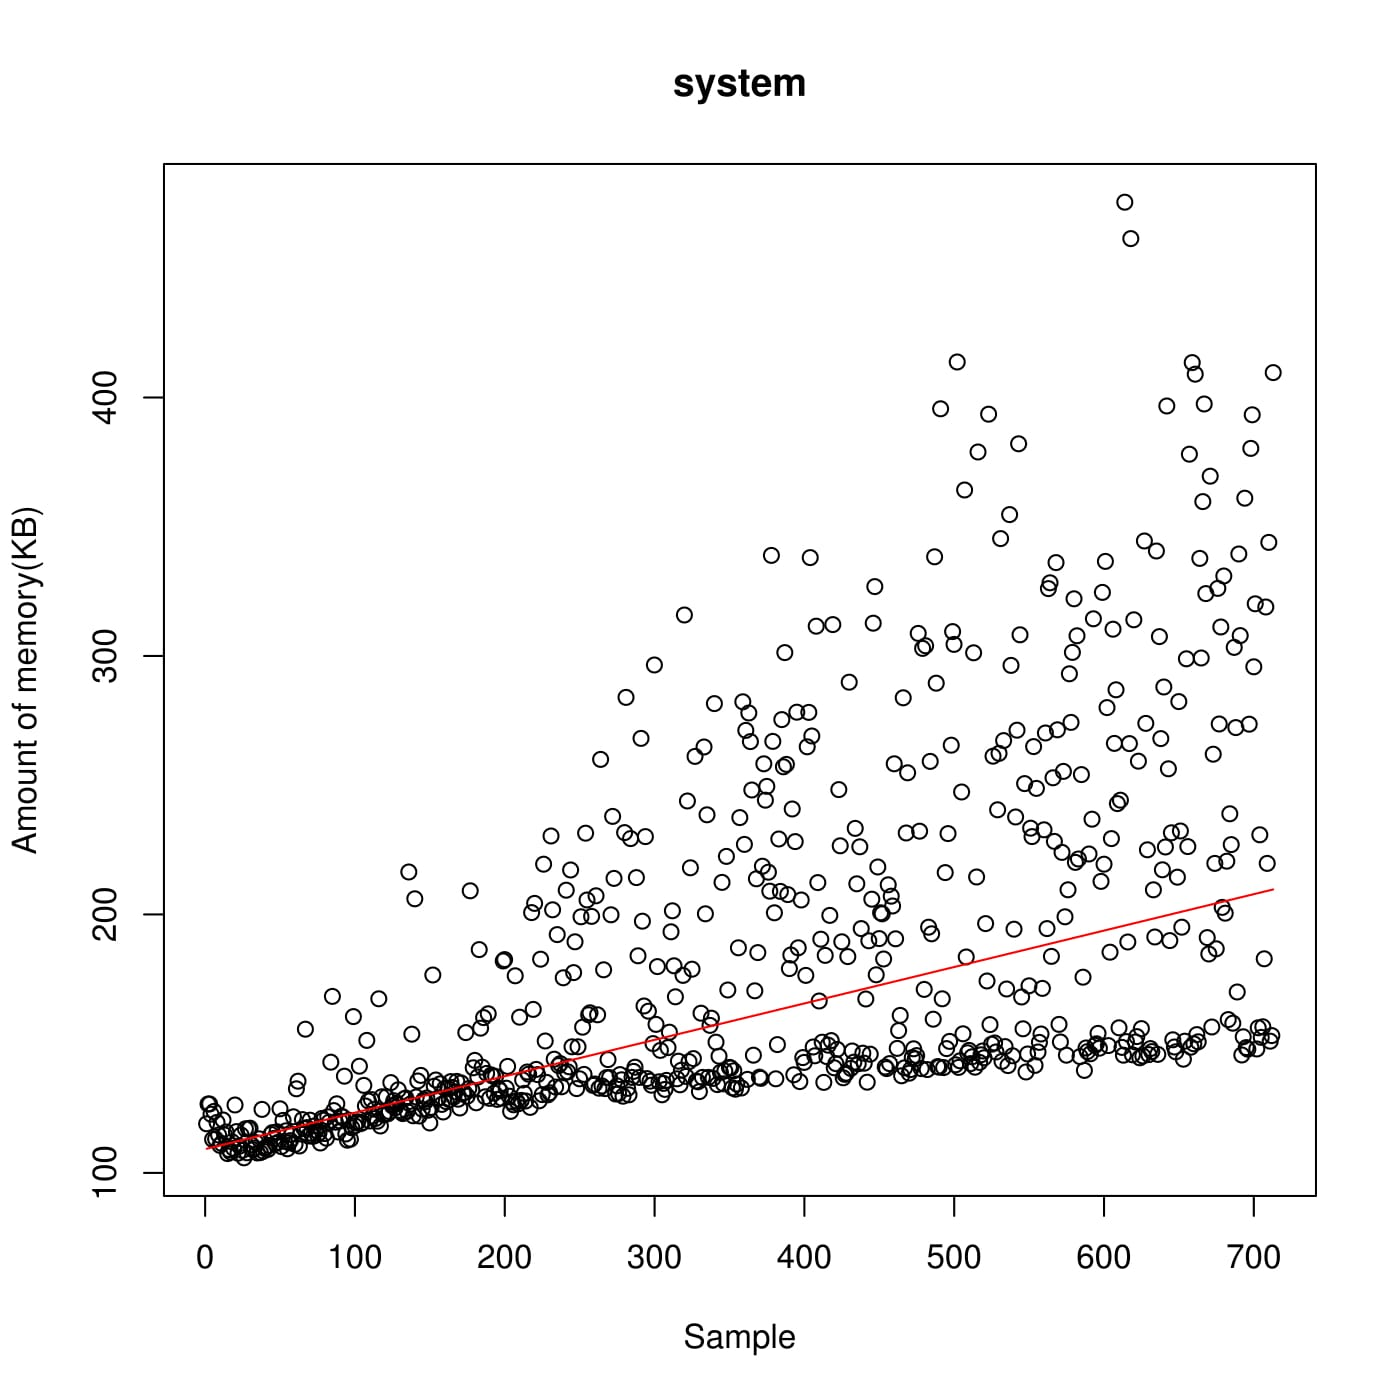
\includegraphics[width=\linewidth]{system_1}
    \end{figure}
  \end{minipage}
  \begin{minipage}{0.49\linewidth}
    \begin{figure}[H]
      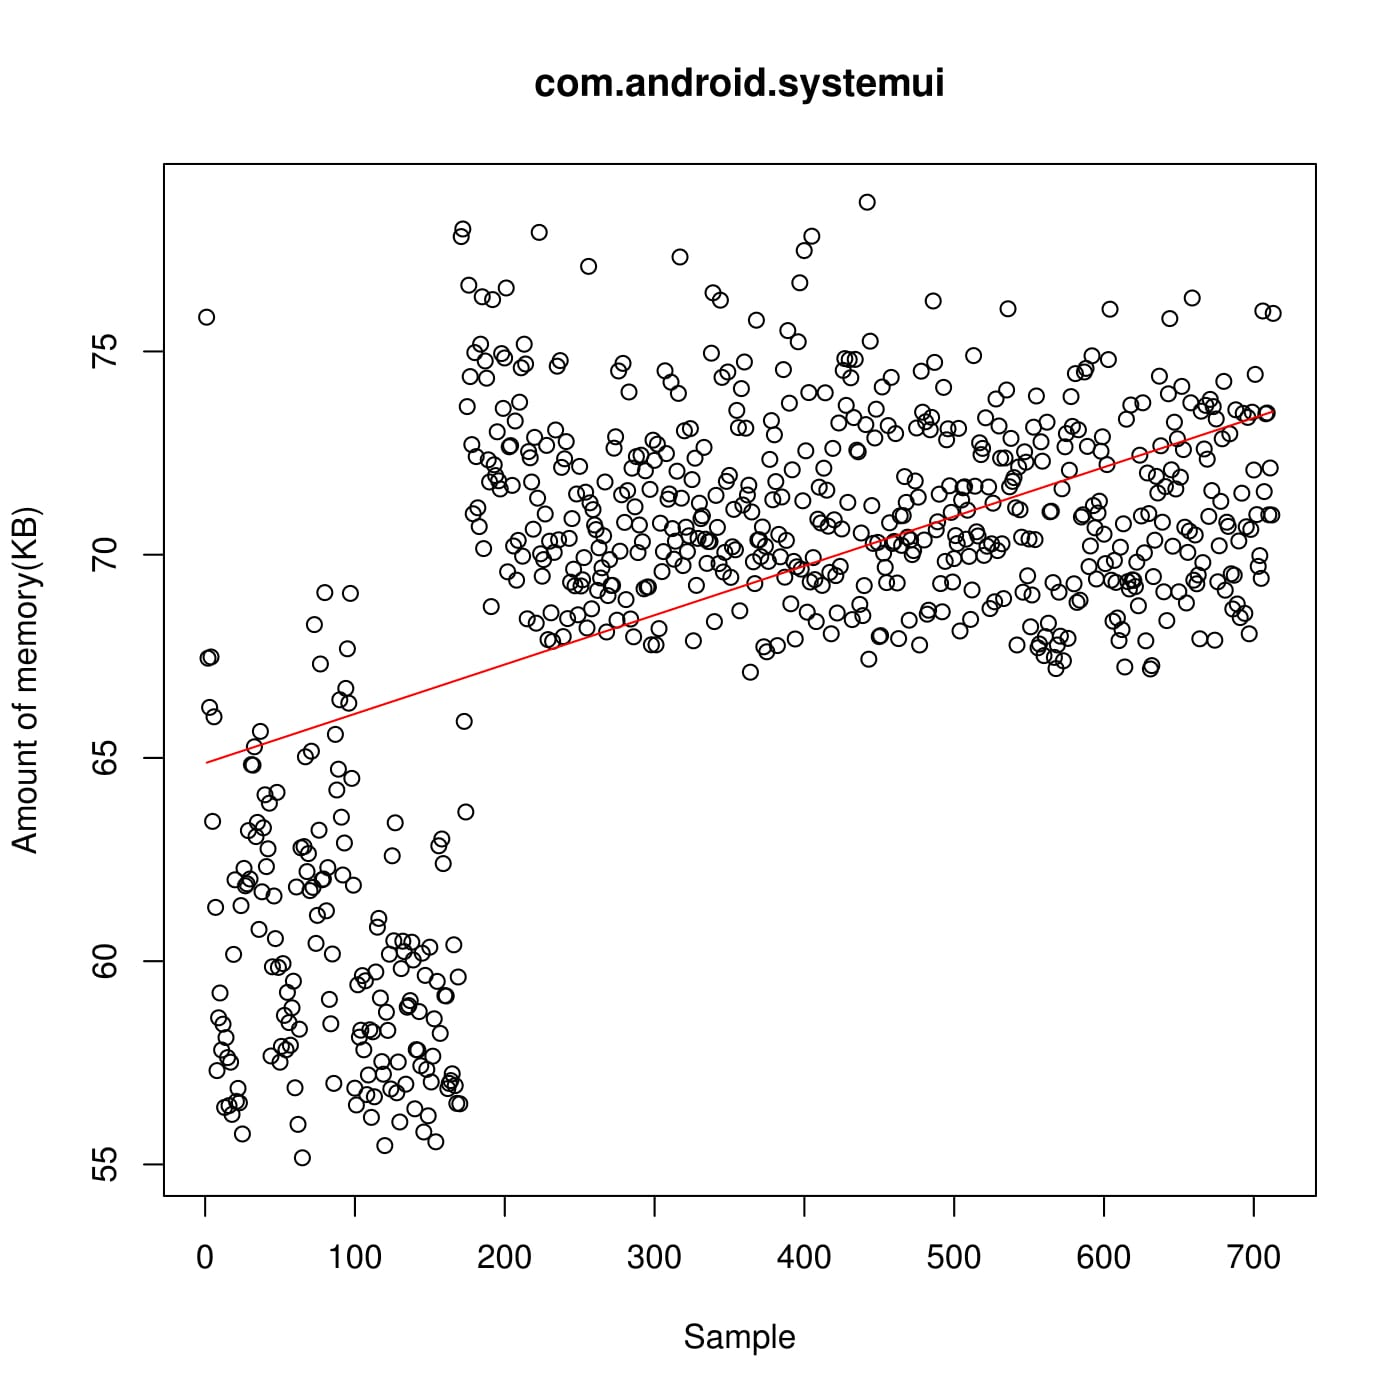
\includegraphics[width=\linewidth]{systemui_1}
    \end{figure}
  \end{minipage}
  \begin{minipage}{0.49\linewidth}
    \begin{figure}[H]
      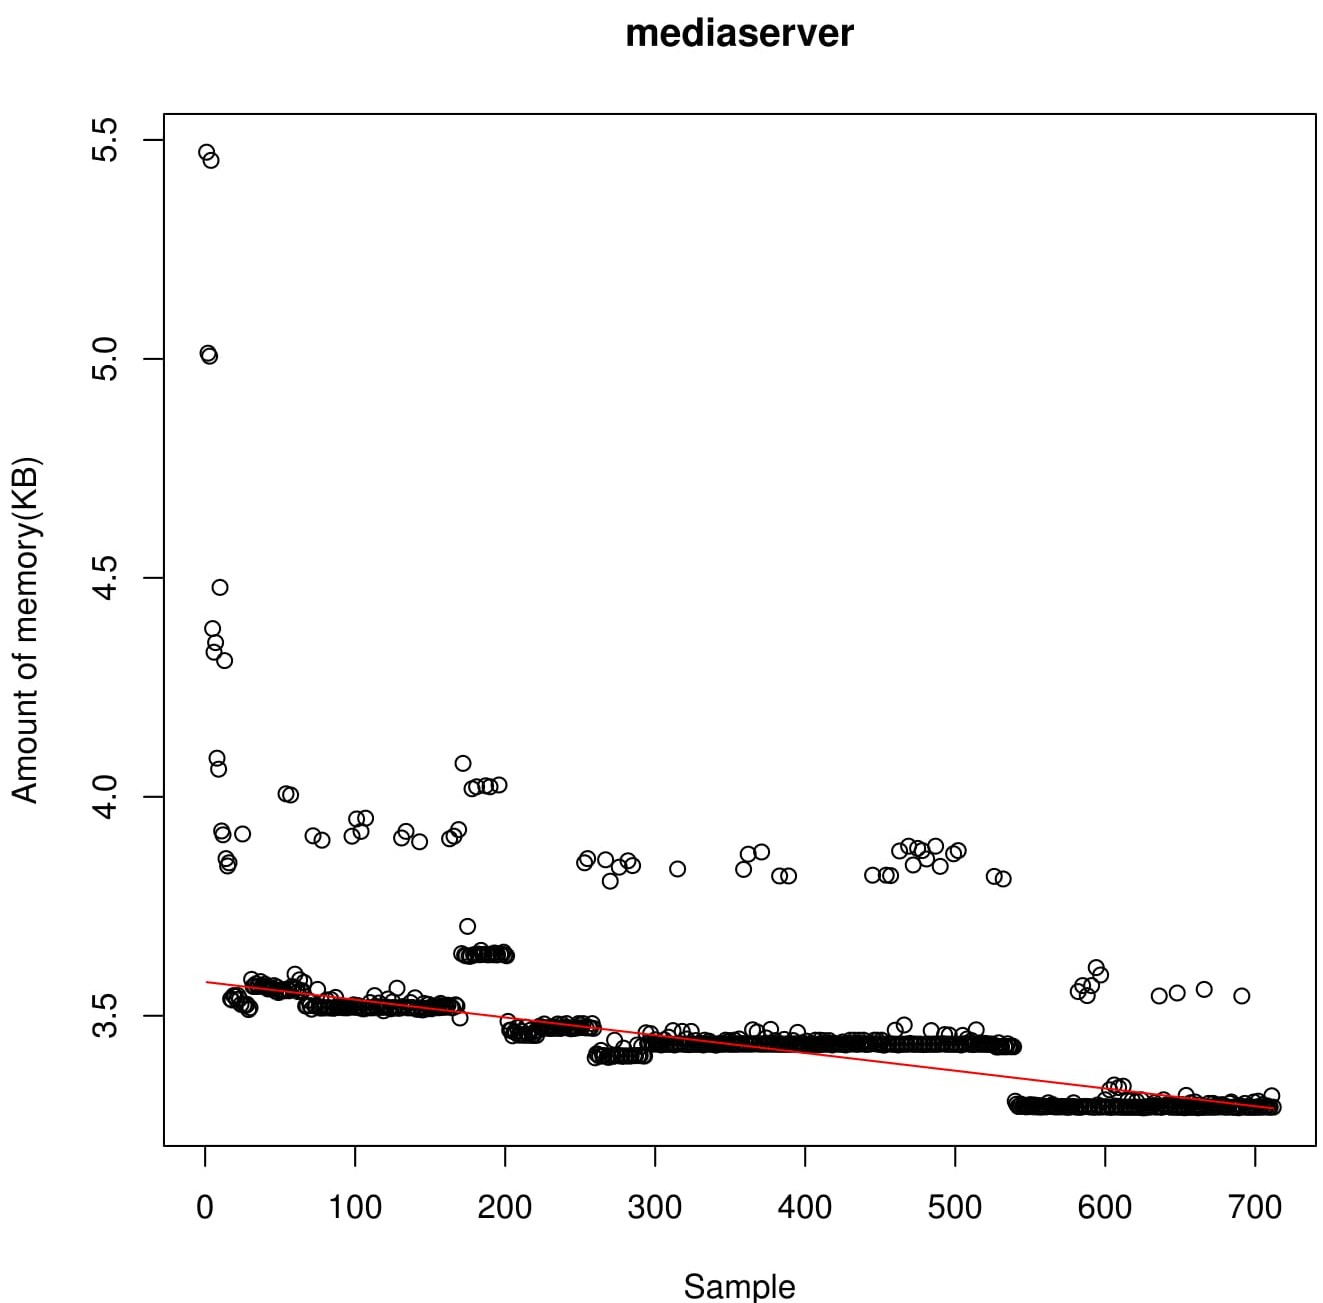
\includegraphics[width=\linewidth]{mediaserver_1}
    \end{figure}
  \end{minipage}
  \begin{minipage}{0.49\linewidth}
    \begin{figure}[H]
      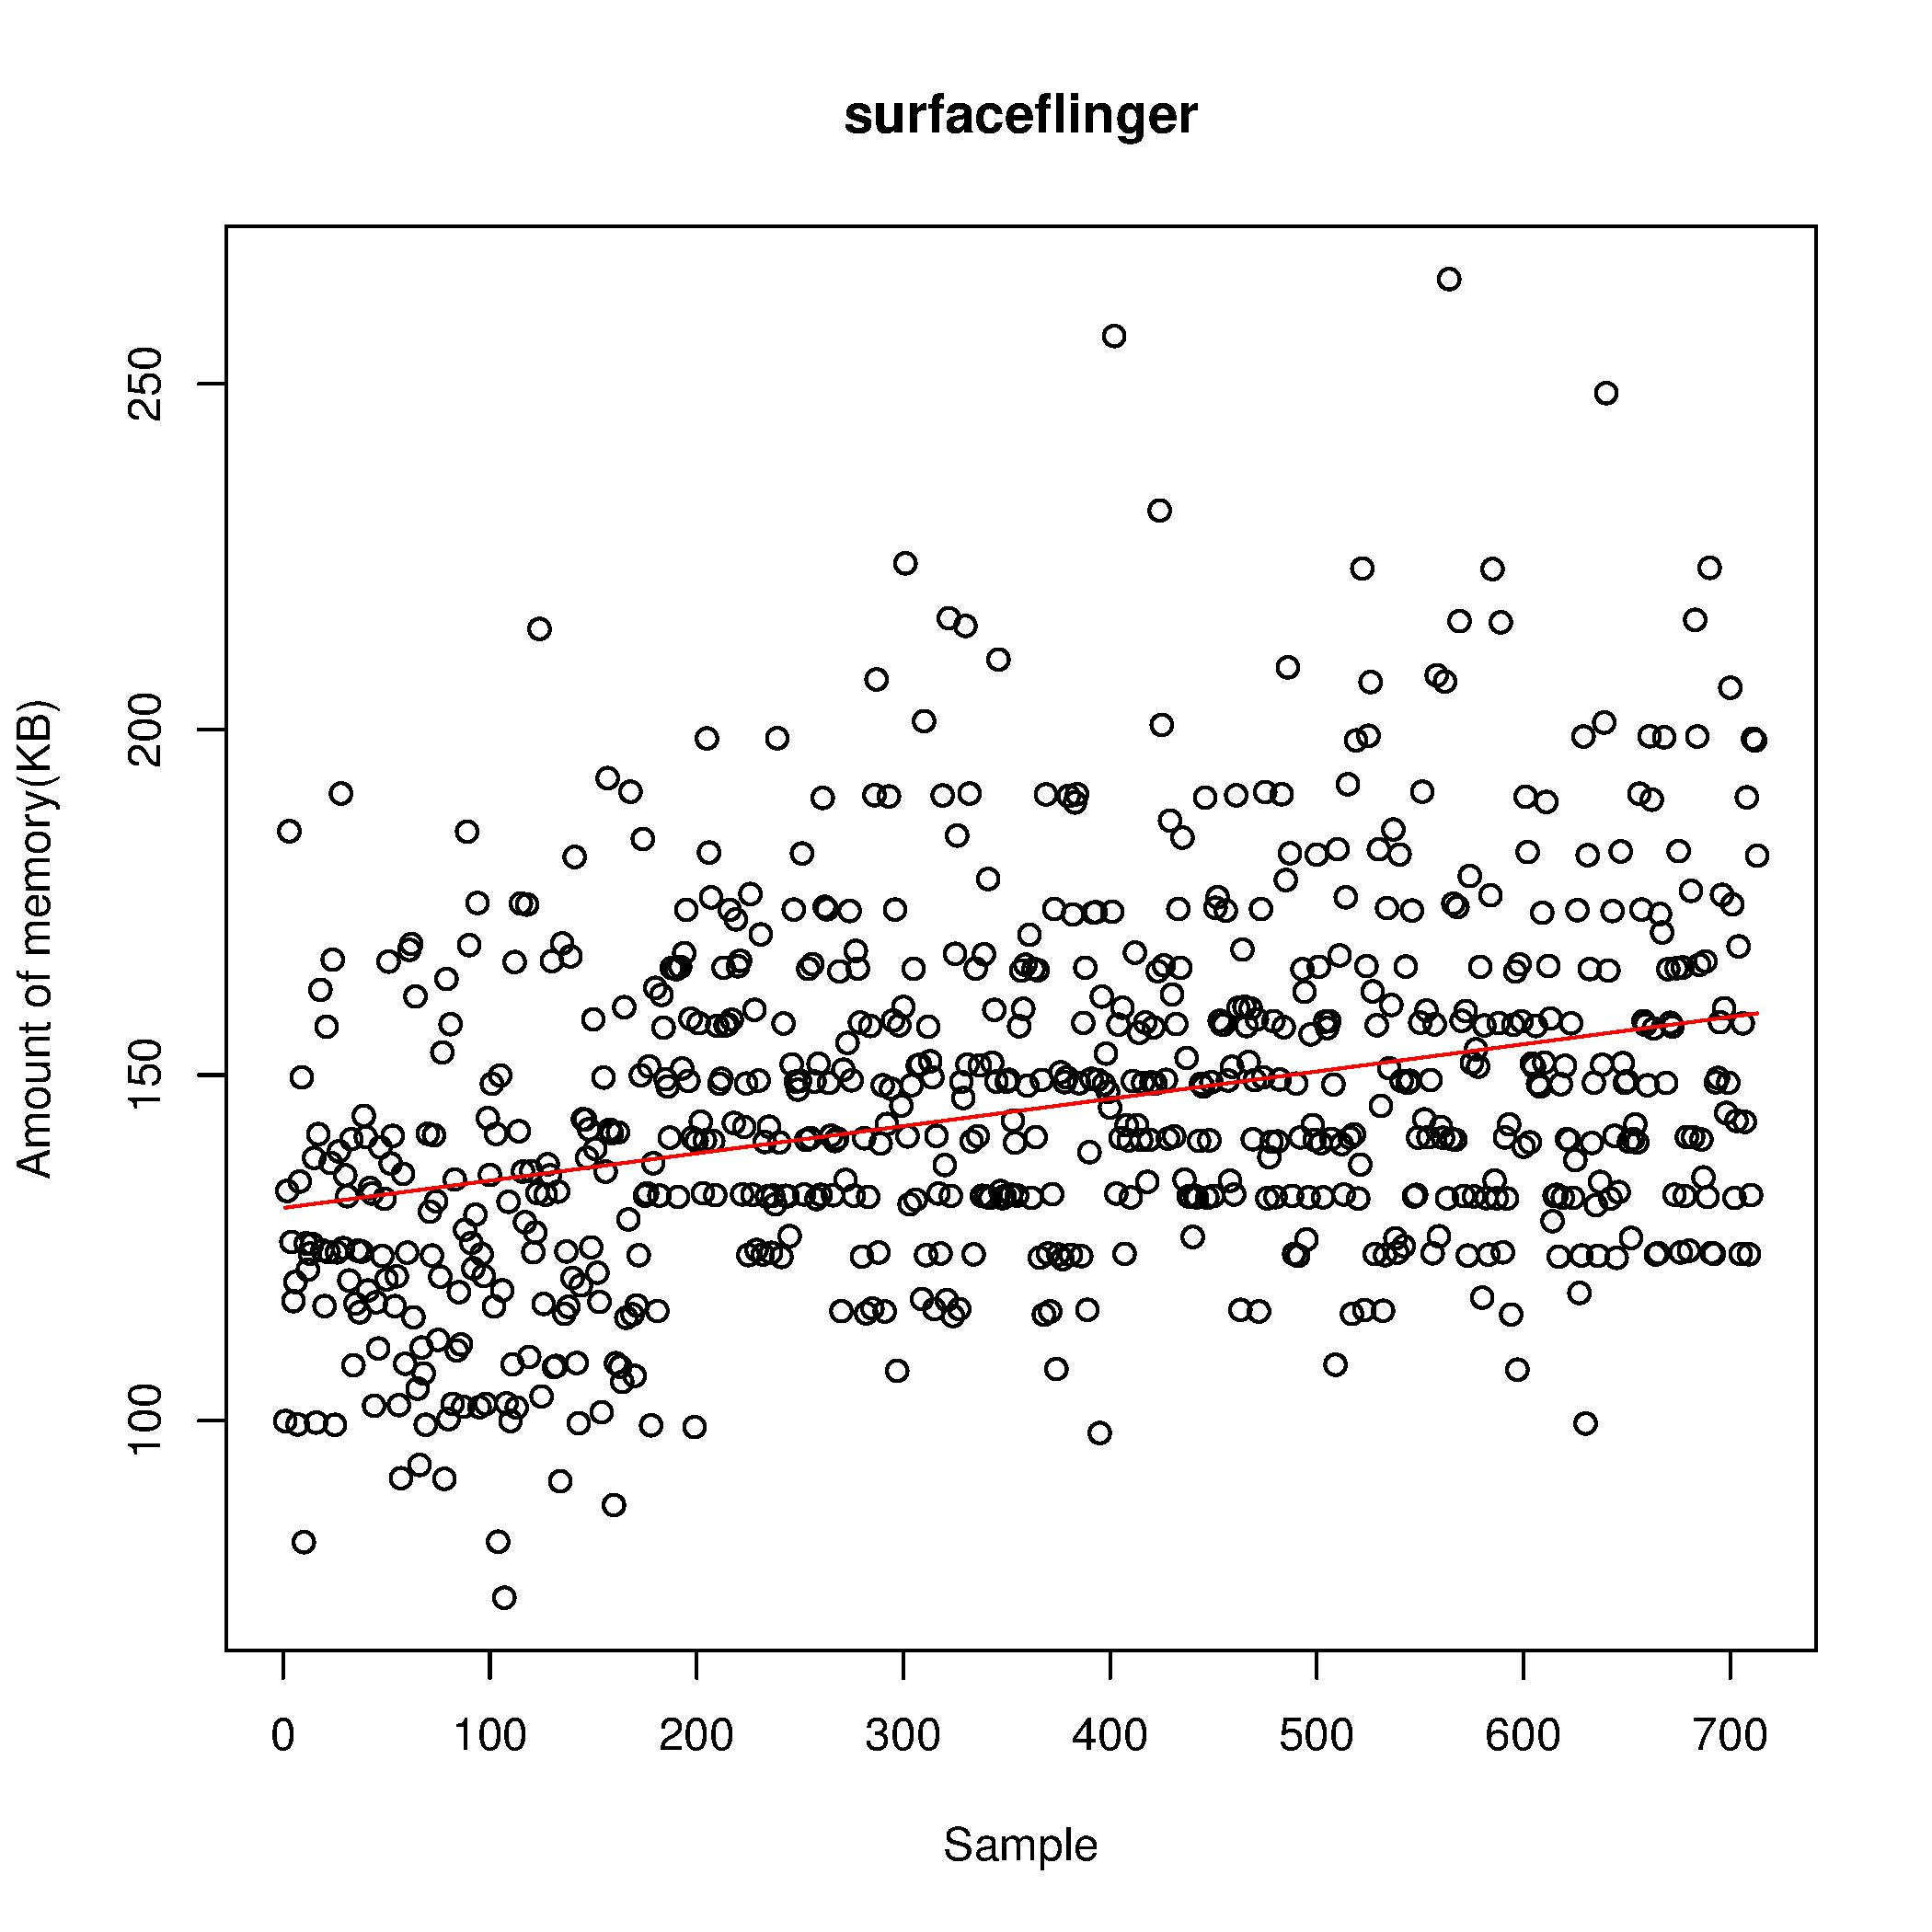
\includegraphics[width=\linewidth]{surfaceflinger_1}
    \end{figure}
  \end{minipage}
\end{minipage}
\captionof{figure}{Trends in system, systemui, mediaserver, surfaceflinger}
\label{and_minipage_trends}

\clearpage
\subsection{Memory Analysis(Worklaod Variable)}

Nell'analisi a basso livello verrà considerato il parametro PSS dei processi \textit{system},
\textit{systemui}, \textit{mediaserver} e \textit{surfaceflinger}, dei quali
sarà verificata l'esistenza di un trend.\\

\begin{figure}[!htbp]
  \centering
  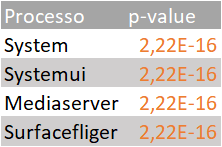
\includegraphics[width=.3\linewidth, keepaspectratio]{pvalue_memoria_1}
  \caption{System}
  \label{and_pvalue_memoria_1}
\end{figure}

Nella tabella in figura \ref{and_pvalue_memoria_1} sono riportati i p-value associati
al \textit{Mann Kendall test}.\\
Quest'ultimo suggerisce che può essere rigettata l'ipotesi nulla, dimostrando
che in tutte le serie temporali esiste un trend.\\
In particolare, osservando le immagini in figura \ref{and_minipage_trends2}, si verifica che effettivamente
tutti i processi presentano un trend, in particolare \textit{mediaserver},
il quale presenta un trend negativo.\\
Il trend più significativo è verificato nei processi \textit{system} e \textit{systemui}.

\begin{minipage}{\linewidth}
  \centering
  \begin{minipage}{0.49\linewidth}
    \begin{figure}[H]
      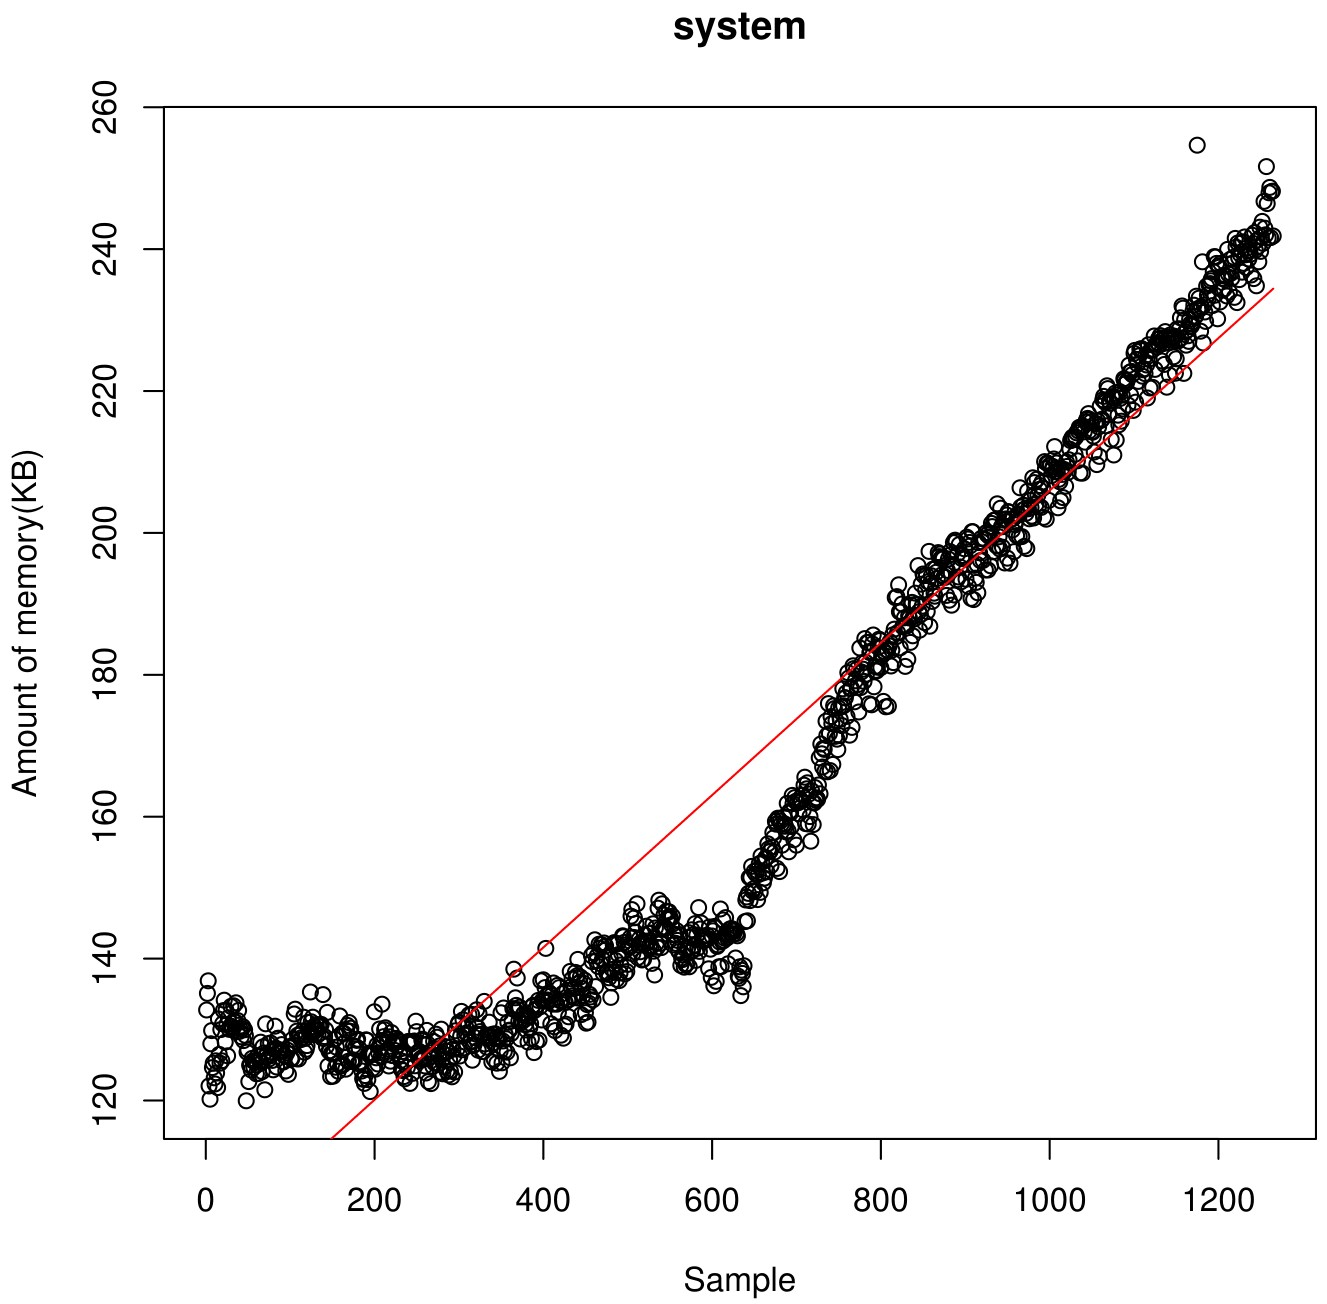
\includegraphics[width=\linewidth]{system_2}
    \end{figure}
  \end{minipage}
  \begin{minipage}{0.49\linewidth}
    \begin{figure}[H]
      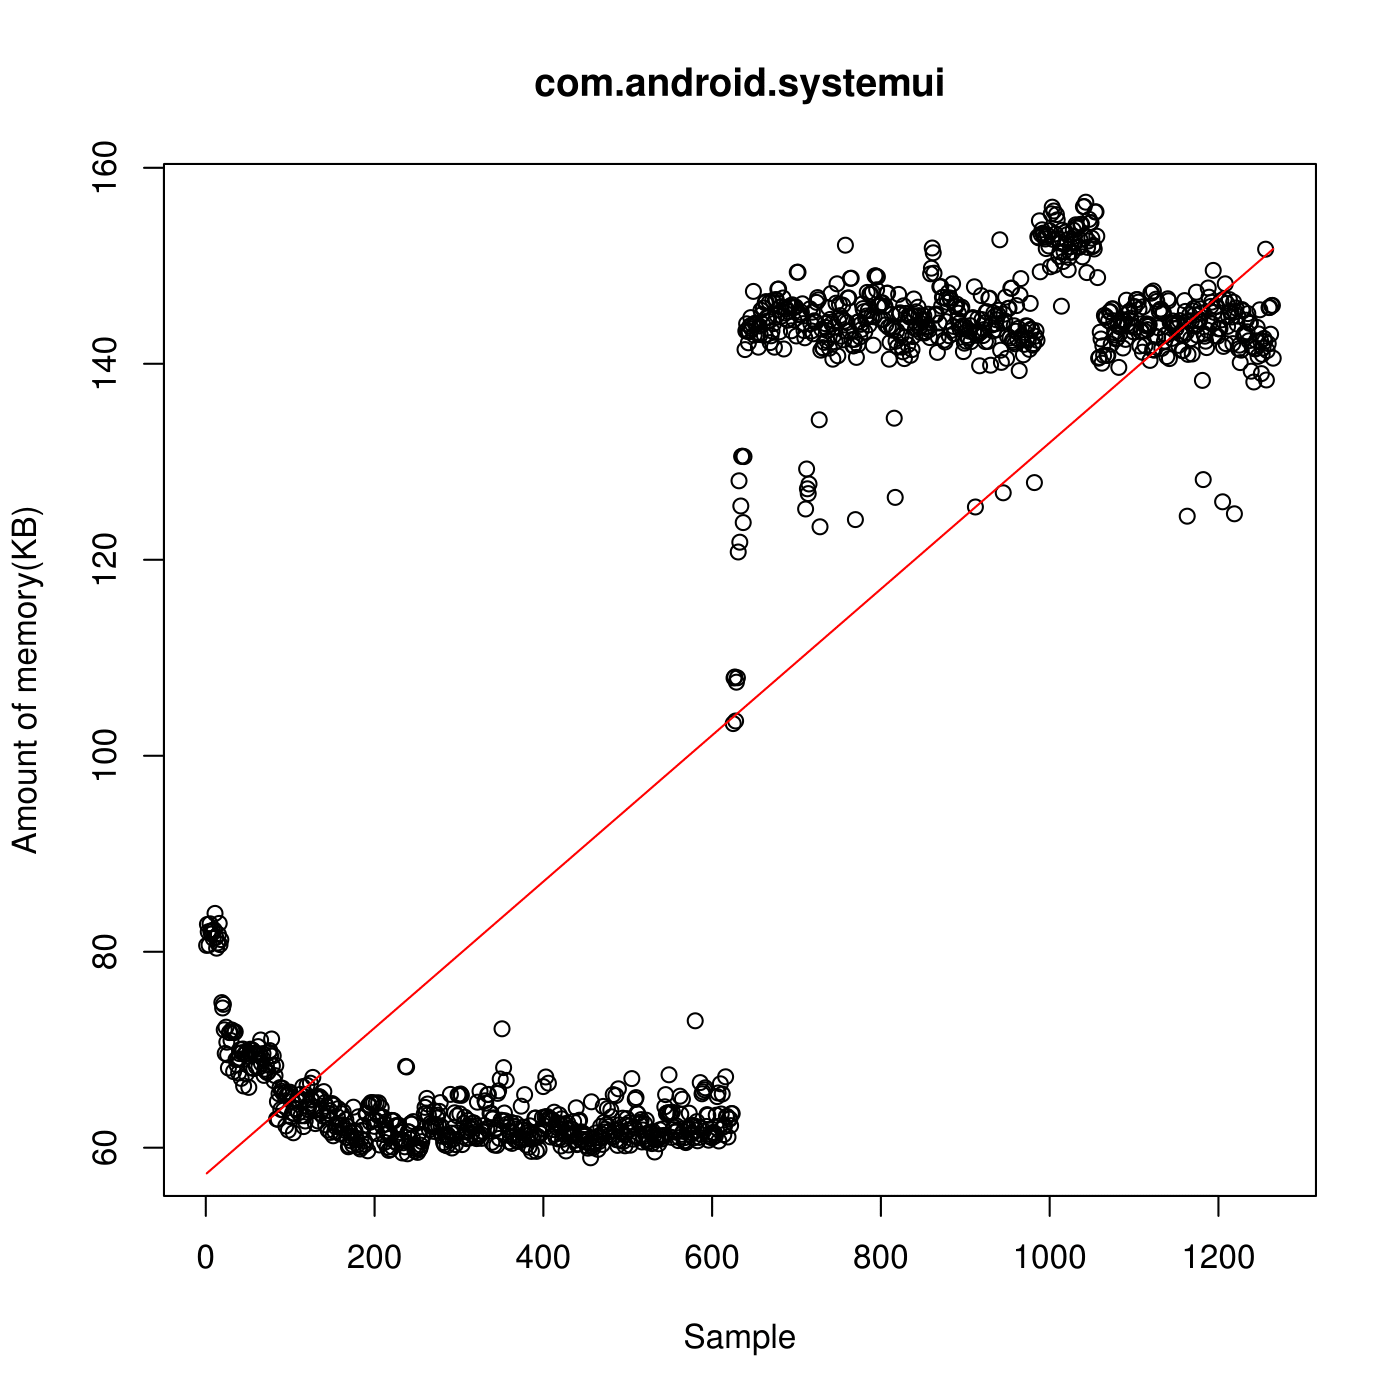
\includegraphics[width=\linewidth]{systemui_2}
    \end{figure}
  \end{minipage}
  \begin{minipage}{0.49\linewidth}
    \begin{figure}[H]
      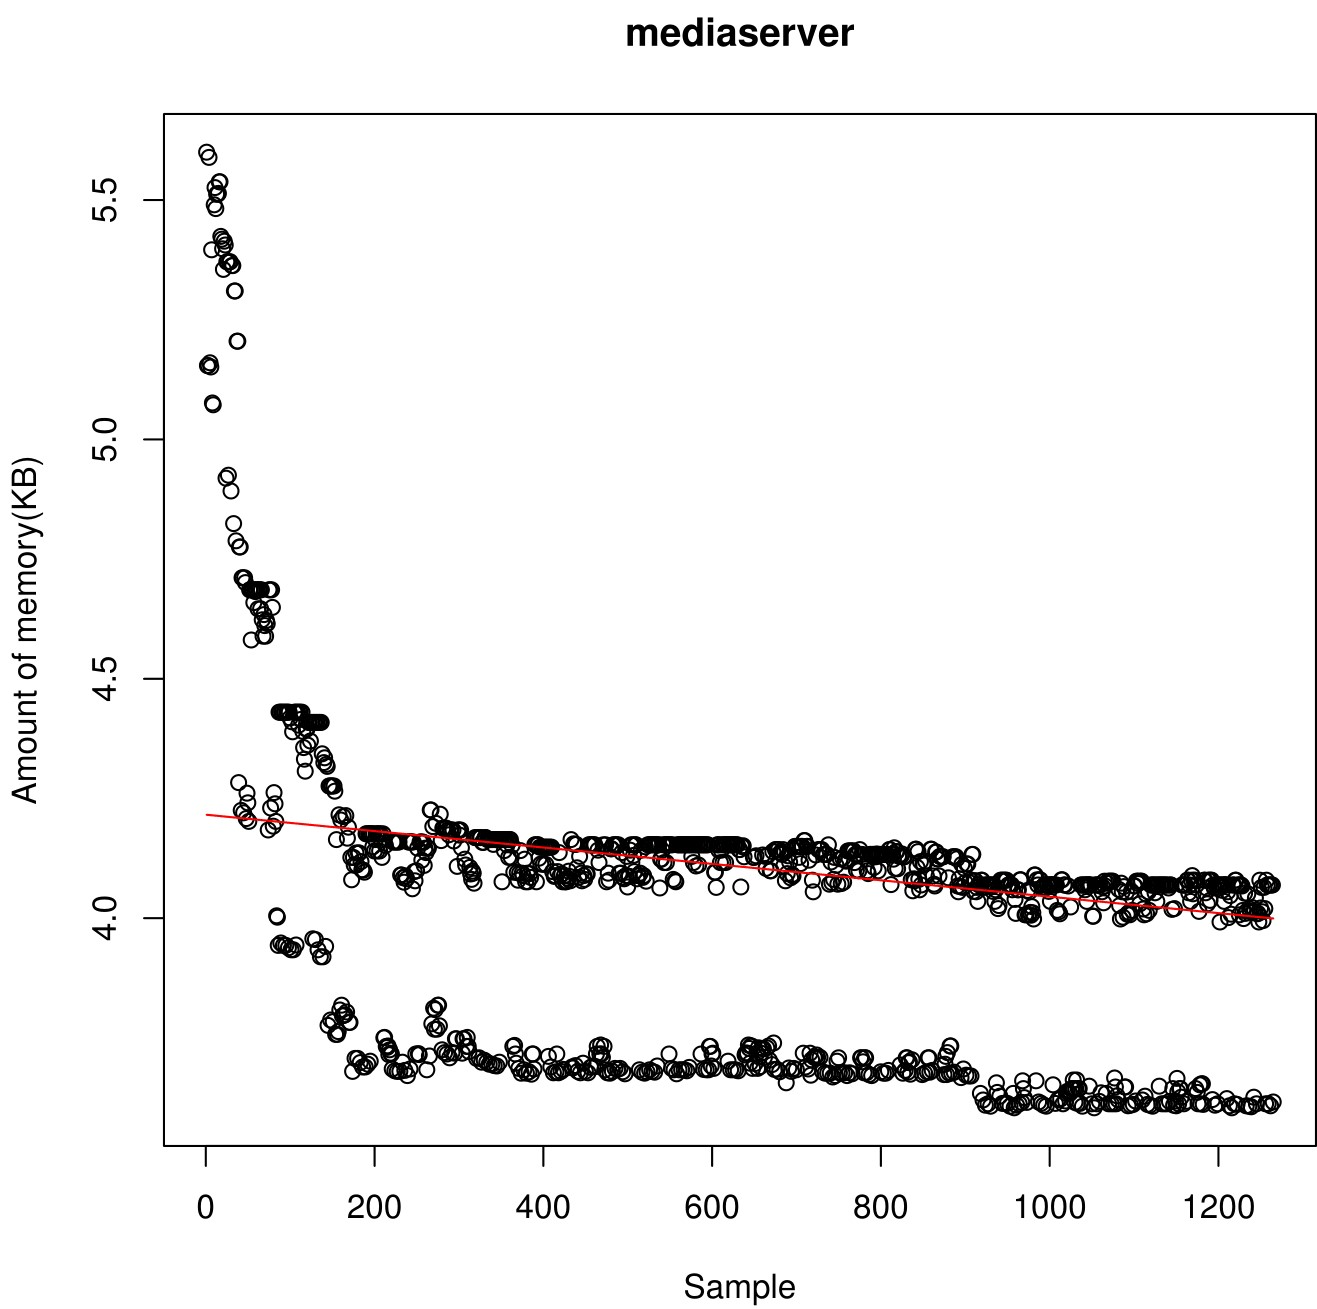
\includegraphics[width=\linewidth]{mediaserver_2}
    \end{figure}
  \end{minipage}
  \begin{minipage}{0.49\linewidth}
    \begin{figure}[H]
      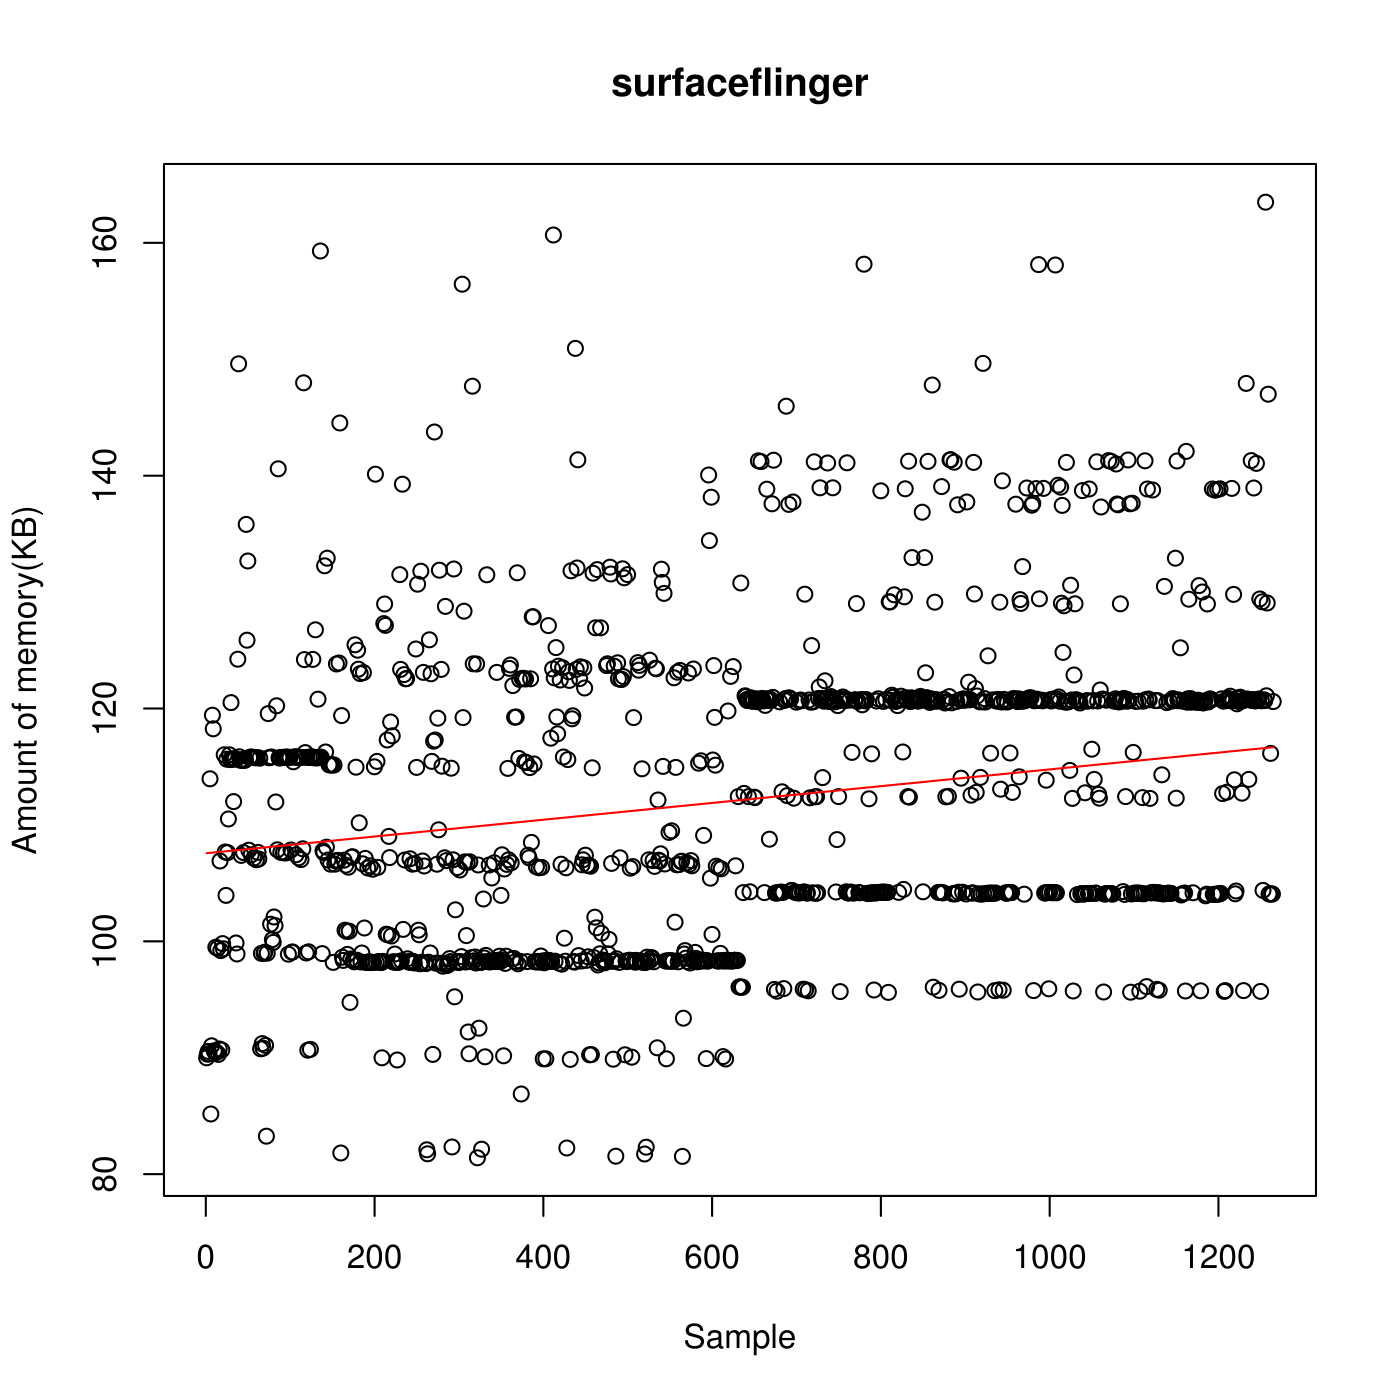
\includegraphics[width=\linewidth]{surfaceflinger_2}
    \end{figure}
  \end{minipage}
\end{minipage}
\captionof{figure}{Trends in system, systemui, mediaserver, surfaceflinger}
\label{and_minipage_trends2}

\clearpage

\section{Relazione causa-effetto}

Per studiare le relazioni causa-effetto tra i KPI della Memoria e il crescere
del PSS del processo \textit{system}, si utilizza la regressione multi-lineare.\\
Saranno analizzate due tecniche:

\begin{itemize}
  \item \textbf{Stepwise Regression}: crea un modello di regressione aggiungendo
  un predittore per volta(forward), oppure iniziando con tutti i predittori
  ed eliminandone uno per volta (backward), esiste anche un approccio misto.\\
  Non elimina la dipendenza lineare, ma conserva i predittori originali;
  \item \textbf{PCA-Based regression}: simile alla precedente, effettua
  una PCA preliminare sui predittori.\\
  Elimina la dipendenza lineare, ma non conserva i predittori originali.
\end{itemize}

\clearpage

\subsection{Stepwise Regression Workload Fixed}

Di seguito è riportato il risultato ottenuto in \textbf{\textit{JMP}} per
la \textit{Stepwise Regression}.\\

\begin{figure}[!htbp]
  \centering
  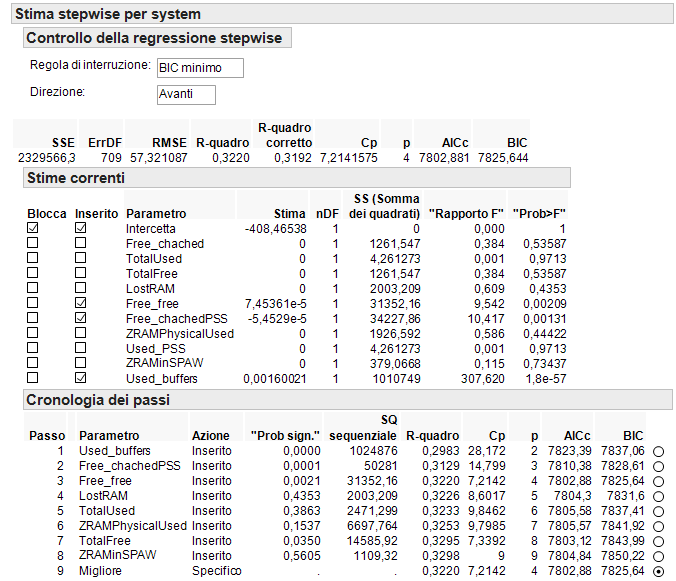
\includegraphics[width=\linewidth, keepaspectratio]{stepwise_1}
  \caption{Stepwise Regression}
  \label{and_stepwise_1}
\end{figure}
\clearpage
Analizzando la figura \ref{and_stepwise_analisi_1}, si osserva che si ha un R-quadro
abbastanza basso, il che significa che la retta di regressione non fitta troppo
bene i dati, mentre l'analisi della varianza(ANOVA) restituisce un p-value basso,
quindi il modello risulta essere significativo.\\
Per quanto riguarda i parametri, si ha che l'intercetta e \textit{Used\_buffer}
sono i parametri più significativi del modello.\\
Questo stesso risultato è visibile anche nel test degli effetti, dove si osserva
che il parametro \textit{Used\_buffer} risulta avere un grande impatto sul modello.\\
\begin{figure}[!htbp]
  \centering
  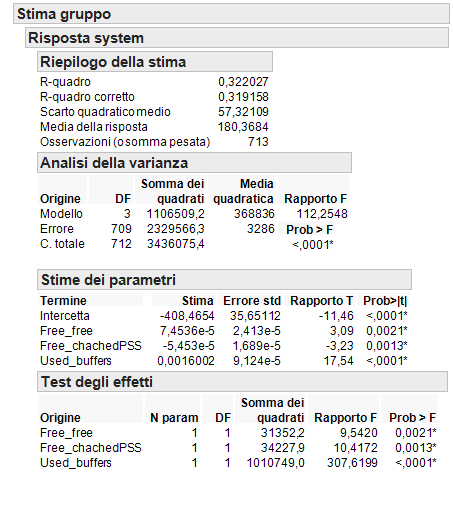
\includegraphics[width=0.7\linewidth, keepaspectratio]{stepwise_analisi_1}
  \caption{Analisi Stepwise Regression}
  \label{and_stepwise_analisi_1}
\end{figure}

\clearpage

\subsection{PCA-Based Regression Workload Fixed}

Per effettuare una \textit{PCA-Based Regression} bisogna applicare la PCA.\\
Di seguito sono riportati i risultati ottenuti in \textbf{\textit{JMP}}.\\

\begin{figure}[!htbp]
  \centering
  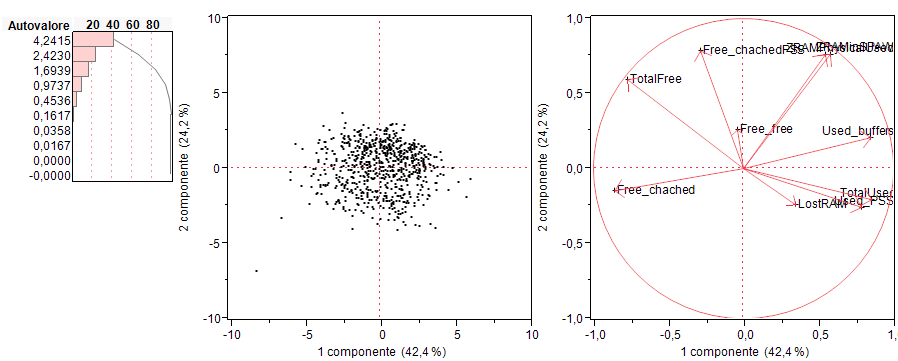
\includegraphics[width=0.85\linewidth, keepaspectratio]{pca_1}
  \caption{Analisi PCA-Based Regression}
  \label{and_pca_1}
\end{figure}

\begin{figure}[!htbp]
  \centering
  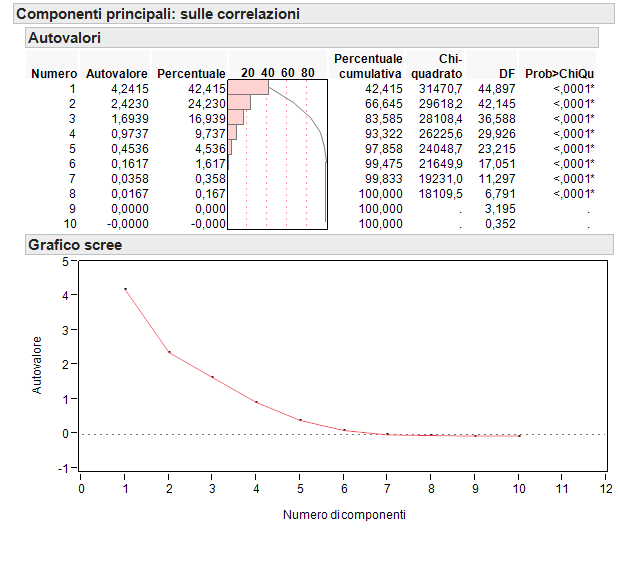
\includegraphics[width=0.7\linewidth, keepaspectratio]{autovalori_1}
  \caption{Analisi PCA-Based Regression}
  \label{and_autovalori_1}
\end{figure}

A valle dell'analisi effettuata in JMP si è scelto di considerare 5 componenti
principali.\\

\clearpage

Di seguito è riportato il risultato ottenuto in \textbf{\textit{JMP}} per
la \textit{PCA-Based Regression}.\\

\begin{figure}[!htbp]
  \centering
  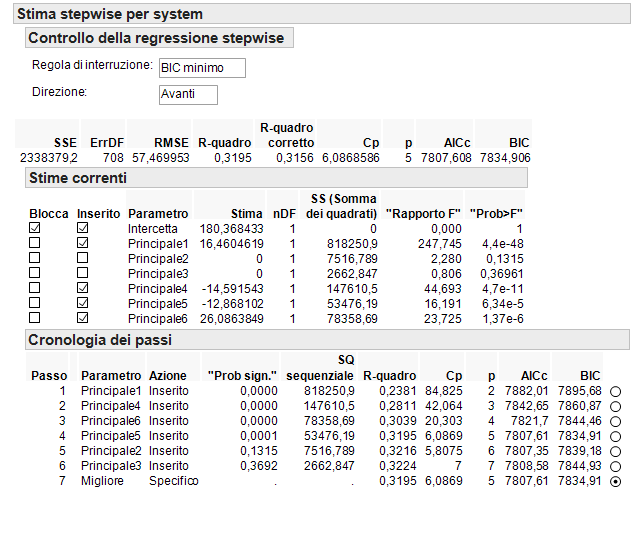
\includegraphics[width=\linewidth, keepaspectratio]{pca_based_1}
  \caption{Analisi PCA-Based Regression}
  \label{and_pca_based_1}
\end{figure}

\clearpage

Analizzando la figura \ref{and_pca_based_analisi_1}, si osserva che si ha un R-quadro
abbastanza basso, il che significa che la retta di regressione non fitta troppo
bene i dati, mentre l'analisi della varianza(ANOVA) restituisce un p-value basso,
quindi il modello risulta essere significativo.\\
In questo caso tutti i parametri sono significativi del modello.\\
Questo stesso risultato è visibile anche nel test degli effetti, dove si osserva
che tutti i parametri risultano avere un grande impatto sul modello.\\

\begin{figure}[!htbp]
  \centering
  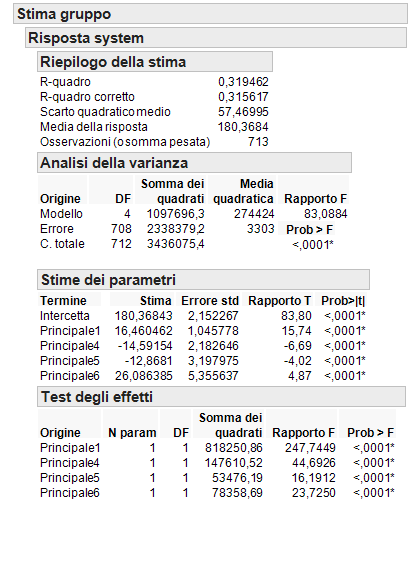
\includegraphics[width=0.7\linewidth, keepaspectratio]{pca_based_analisi_1}
  \caption{Analisi PCA-Based regression}
  \label{and_pca_based_analisi_1}
\end{figure}

\clearpage

\subsection{Stepwise Regression Workload Variable}

Di seguito è riportato il risultato ottenuto in \textbf{\textit{JMP}} per
la \textit{Stepwise Regression}, nel caso di workload variabile.\\

\begin{figure}[!htbp]
  \centering
  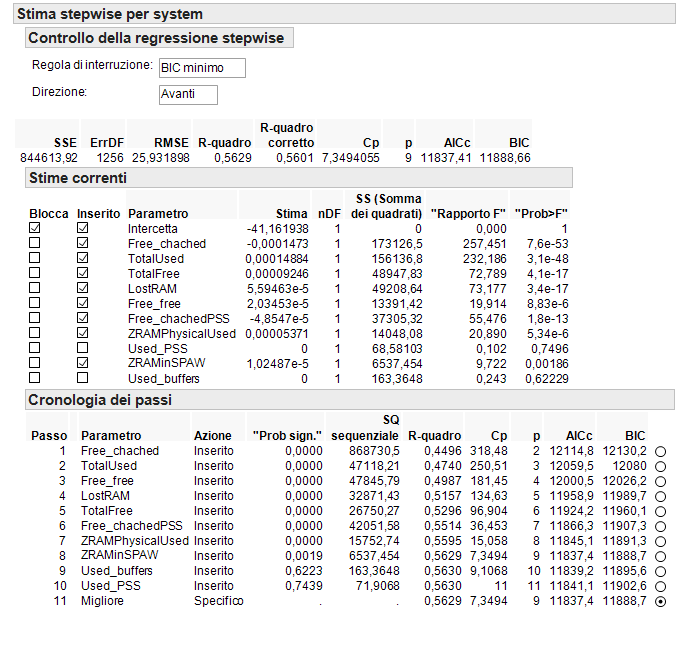
\includegraphics[width=\linewidth, keepaspectratio]{stepwise_2}
  \caption{Stepwise Regression}
  \label{and_stepwise_2}
\end{figure}
\clearpage
Analizzando la figura \ref{and_stepwise_analisi_2}, si osserva che si ha un R-quadro
abbastanza basso, il che significa che la retta di regressione non fitta troppo
bene i dati, mentre l'analisi della varianza(ANOVA) restituisce un p-value basso,
quindi il modello risulta essere significativo.\\
Per quanto riguarda i parametri, si ha che tutti i parametri risultano essere
significativi, a meno di intercetta e \textit{ZRAMinSWAP}.\\
Questo stesso risultato è visibile anche nel test degli effetti, dove si osserva
che tutti i parametri risultano avere un grande impatto sul modello, eccezion
fatta per \textit{ZRAMinSWAP}.\\
\begin{figure}[!htbp]
  \centering
  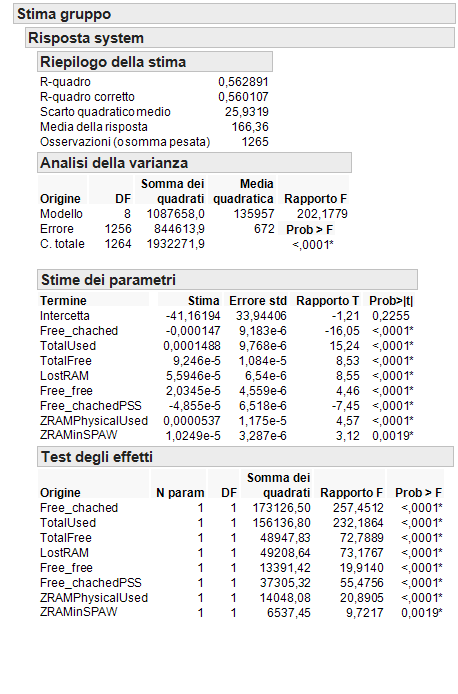
\includegraphics[width=0.7\linewidth, keepaspectratio]{stepwise_analisi_2}
  \caption{Analisi Stepwise Regression}
  \label{and_stepwise_analisi_2}
\end{figure}

\clearpage

\subsection{PCA-Based Regression Workload Fixed}

Per effettuare la \textit{PCA-Based Regression} bisogna applicare la PCA.\\

\begin{figure}[!htbp]
  \centering
  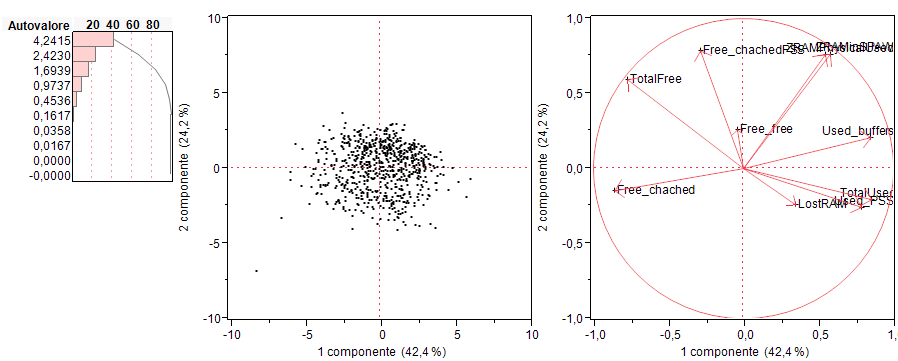
\includegraphics[width=0.85\linewidth, keepaspectratio]{pca_1}
  \caption{Analisi PCA-Based Regression}
  \label{and_pca_2}
\end{figure}

\begin{figure}[!htbp]
  \centering
  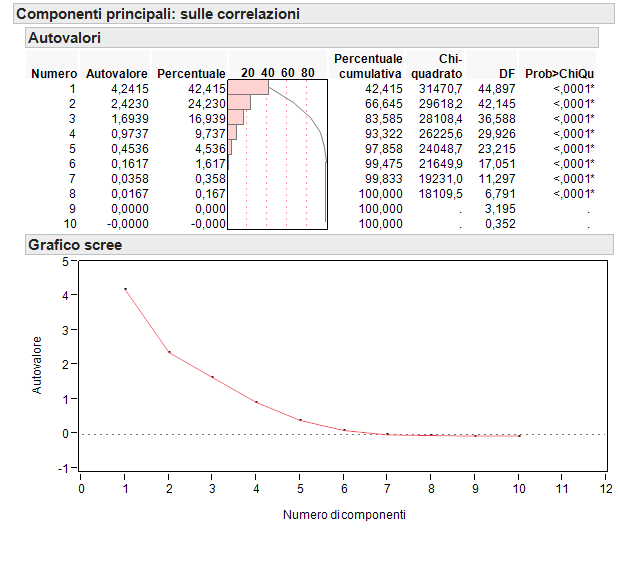
\includegraphics[width=0.7\linewidth, keepaspectratio]{autovalori_1}
  \caption{Analisi PCA-Based Regression}
  \label{and_autovalori_2}
\end{figure}

A valle dell'analisi effettuata in JMP si è scelto di considerare 7 componenti
principali.\\

\clearpage

Di seguito è riportato il risultato ottenuto in \textbf{\textit{JMP}} per
la \textit{PCA-Based Regression}.\\

\begin{figure}[!htbp]
  \centering
  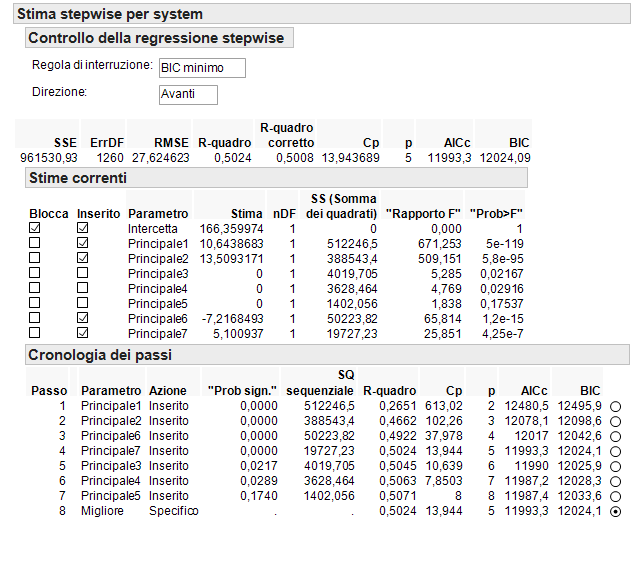
\includegraphics[width=\linewidth, keepaspectratio]{pca_based_2}
  \caption{Analisi PCA-Based Regression}
  \label{and_pca_based_2}
\end{figure}

\clearpage

Analizzando la figura \ref{and_pca_based_analisi_2}, si osserva che si ha un R-quadro
abbastanza basso, il che significa che la retta di regressione non fitta troppo
bene i dati, mentre l'analisi della varianza(ANOVA) restituisce un p-value basso,
quindi il modello risulta essere significativo.\\
In questo caso tutti i parametri sono significativi del modello.\\
Questo stesso risultato è visibile anche nel test degli effetti, dove si osserva
che tutti i parametri risultano avere un grande impatto sul modello.\\

\begin{figure}[!htbp]
  \centering
  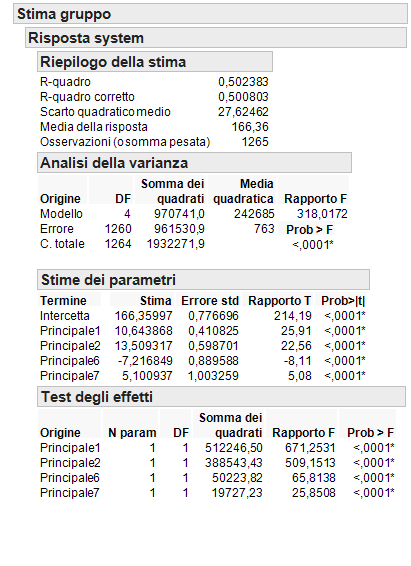
\includegraphics[width=0.7\linewidth, keepaspectratio]{pca_based_analisi_2}
  \caption{Analisi PCA-Based Regression}
  \label{and_pca_based_analisi_2}
\end{figure}
